\chapter{Classifying Tables Describing Comparisons}
\label{table_classification}
A lot of valuable information about comparisons with some baselines and other research is present in the tables of academic research. Researchers tend to spend much valuable time finding the citations and the table of results from those citations. Sci-Genie via Citation Graph and the Machine Learning models filters tables describing comparisons at the time of reading research. 

This chapter will cover the approaches applied to tackle the problem of classifying tables describing comparisons.

\section{Problem Formulation}

The structure of the tables in scientific research can fluctuate based on the information presented by the tables. The tables may also contain information whose context cannot be exactly inferred without the caption underneath the table. Tables occurring in scientific research can also be segregated into well-defined types such as the ones described in Chapter \ref{relatedwork:table-type}. These tables may also not contain a directly linkable entity from a knowledge base(KB) as entities defined in the research may not be present in the KB. Due to such different intrinsic characteristics, models trained using knowledge bases along with web tables such as the one by \cite{deng2020turl} cannot be directly fit to solve this problem.

\begin{table}
    \label{table\arabic{tablecounter}}
    \centering
    \begin{tabular}{|l|l|l|}
        \hline
        Symbol & Meaning & Type \\ \hline
        $Y$ & Labels & Discrete : $\{0,1\}$ \\ \hline
        $X_T$ & Cell Embedding & $\mathbb{R}^{T_l \times d}$\\ \hline
        $X_C$ & Caption Embedding & $\mathbb{R}^{C_l \times d}$ \\ \hline
        $P_C$ & Positional Embedding & $\mathbb{R}^{C_l \times d}$ \\ \hline
        $E_r$ & Row Embedding & $\mathbb{R}^{T_l \times d}$ \\ \hline
        $E_c$ & Column Embedding & $\mathbb{R}^{T_l \times d}$ \\ \hline
        $T_l$ & Number Of Cells & $\mathbb{N}$ \\ \hline
        $T_r$ & Number Of Rows & $\mathbb{N}$ \\ \hline
        $T_c$ & Number Of Columns & $\mathbb{N}$ \\ \hline
        $C_l$ & Length of Caption & $\mathbb{N}$ \\ \hline
        $T_{cell}$ & Sequnces of Cells & $\mathbb{N}^{T_l}$ \\ \hline
        $f_\theta$ & Neural Network & - \\ \hline
    \end{tabular}
    \caption{\label{tablecounter} Table Of Symbols for Equations. }
\end{table}
\refstepcounter{tablecounter}
The problem of classifying a table $T$ as a table describing a comparison can be framed as a binary classification problem. Given a table $T$ and its caption $C$, the classifier $f_\theta(T,C) \rightarrow Y$ predicts a binary label $Y \in \{0,1\}$ to denote weather the table is describing a comparison of entities\footnote{Both the table and caption are used because human labeling discovered that these two variables combined are the most prominant indicators of a table describing a comparison.}. 

Based on this formulation, this dissertation analyzes 4 different types of ML models and the representations they use for the table $T$ and caption $C$ for the problem:
\begin{itemize}
    \item Cross Channel Transformers(CC-T) With/Without Pretraining
    \item Encoder Only Multi-Channel Transformer(E-MCT) With/Without Pretraining
    \item Caption only Encoder Transformer With/Without Pretraining 
    \item Finetuning Pretrained Scibert (Baseline)
    \item SVM and Naive Bayes (Baseline)
\end{itemize}

\begin{figure}[h]
    \centering
    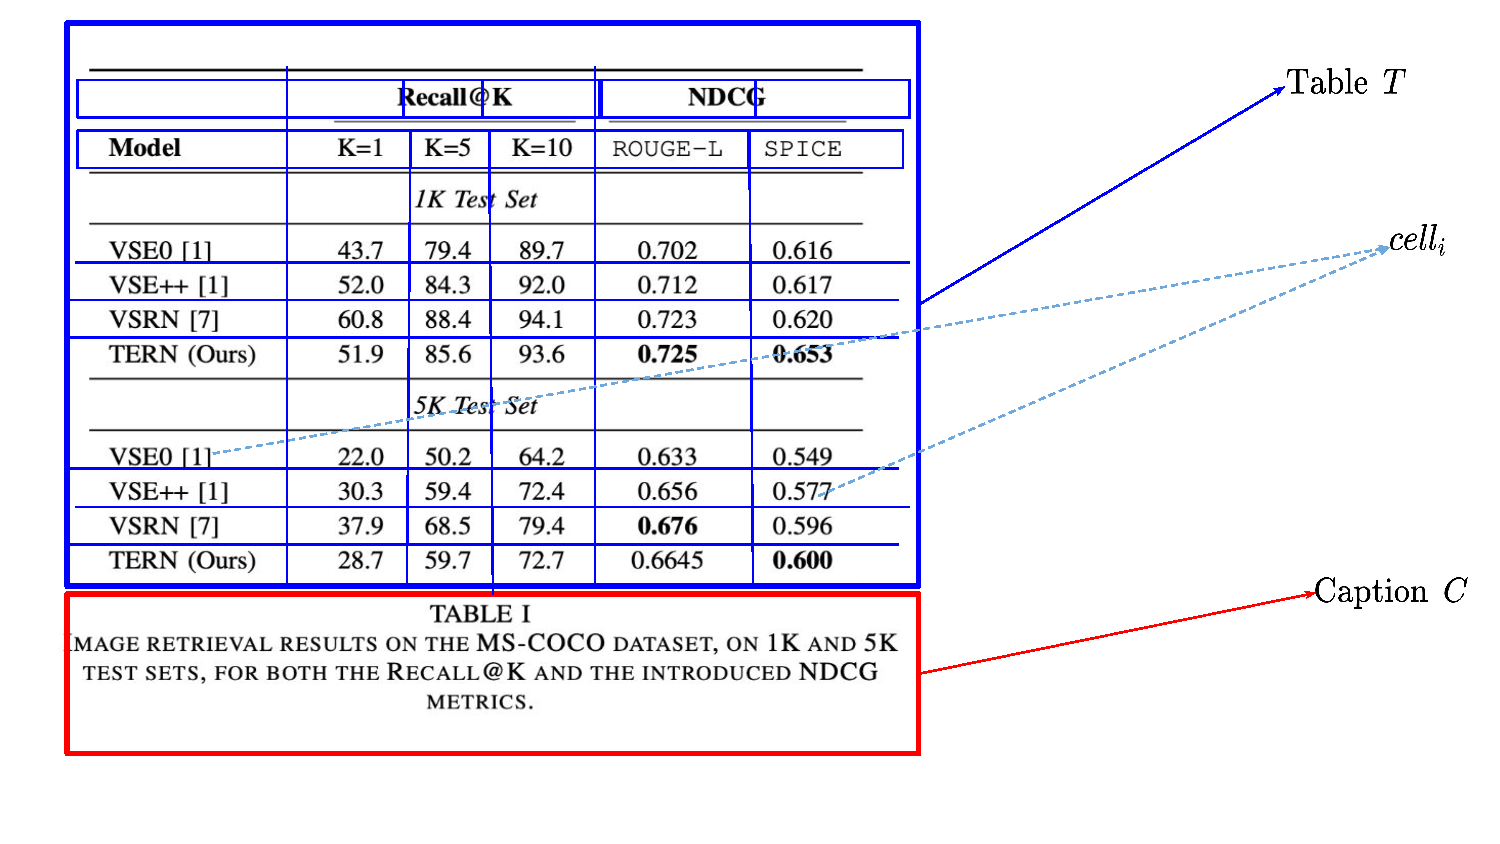
\includegraphics[width=\maxwidth{\textwidth}]{src/images/table-structure.pdf}
    \caption{An example representation of Table $T$ and Caption $C$. Each Table $T$ consists of sequence of $cell$'s. }
    \label{figure\arabic{figurecounter}}
\end{figure}
\refstepcounter{figurecounter}

Figure \ref{figure17} visualizes the representation of $T$ and $C$. Different models are analyzed because the representations of $T$ and $C$ can be treated as seperate variables or as a single variable, based on the choice of the model. Cross Channel Transformer and Encoder Only Multi-Channel Transformer treats $T$ and $C$ as separate representations. Scibert treats $T$ and $C$ as one joint representation. The caption only transformer only uses the Caption $C$. The caption only transformer is tested, to validate the hypothesis of wheather only captions themselves can be enough for classifying tables describing comparisons. 

Section \ref{table_classification:models} describes the models developed/trained for the input representations of table $T$ and caption $C$. The data collection and labeling for the machine learning models is described in Section \ref{table_classification:data-coll}. The experiment results for different models is described in Section \ref{table_classification:experiment-result}

\section{Classification Models}
\label{table_classification:models}

\subsection{Encoder Only Multi-Channel Transformer (E-MCT)}
\label{table_classification:models:encoder-model}
\begin{figure}[h]
    \centering
    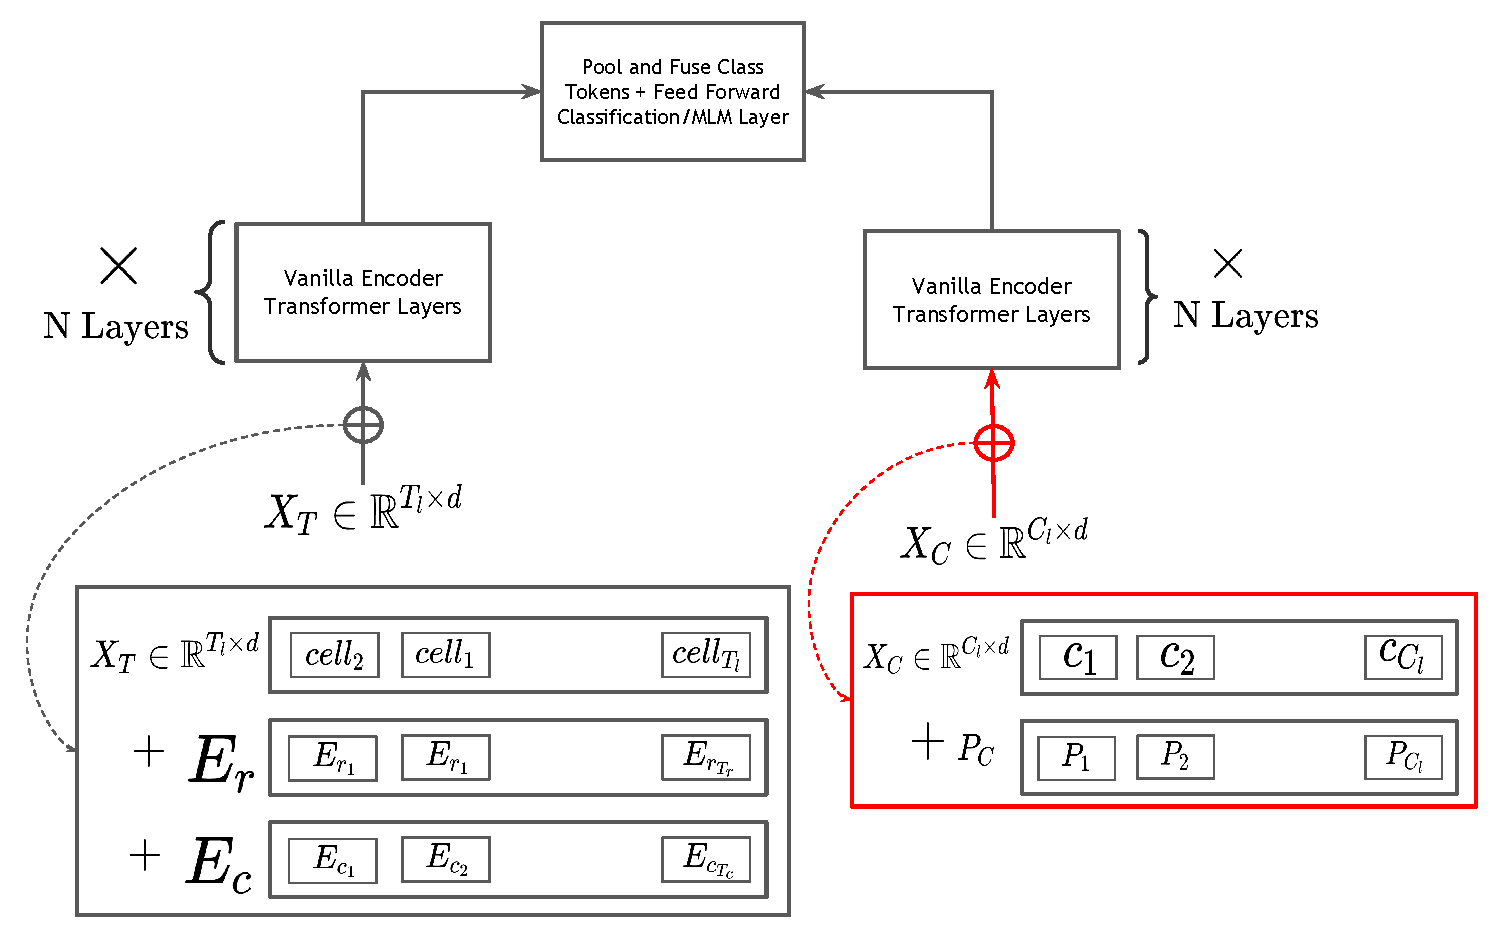
\includegraphics[width=\maxwidth{\textwidth}]{src/images/Pic-Export-Enc-Trans-Thesis.pdf}
    \caption{Encoder Only Multi-Channel Transformer For Table Classification. }
    \label{figure\arabic{figurecounter}}
\end{figure}
\refstepcounter{figurecounter}
Based on the models developed by \cite{deng2020turl}. A structurally-aware encoder only Transformer model is adapted to fit the function $f_\theta$. Figure \ref{figure18} visualizes the model and its input representations.

\subsubsection{Input Representation}
\label{table_classification:models:encoder-model:input-rep}
Each table $T$ is represented as tuple of $(T_{cell},E_r,E_c)$; where $T_{cell} \in \mathbb{N}^{T_l}$ are the cells of the table represented as a sequence of integer tokens; $E_r$ is the row embedding where embedding $E_{r_{i}}$ represents the row of the cell $T_{cell_{i}}$ as an embedding;  $E_c$ is the column embedding where an embedding $E_{c_{i}}$ represents the column of the cell $T_{cell_{i}}$ as an embedding. The caption $C$ is represented as sequence of integer tokens that gets transformed to a sequence of embeddings. The representations for the table $T$ are inspired from the models created by \cite{deng2020turl}. 

The cell sequence tokens $T_{cell}$ and caption $C$ are created using a word-piece tokenizer from the SciBert Model \footnote{https://huggingface.co/allenai/scibert\_scivocab\_uncased}. The tokenizer converts the value of individual cells or the caption into a sequence of integer tokens. These tokens can be used to create embeddings which are passed to the transformer model. 

\subsubsection{Model Description}
The table cell sequence $T_{cell}$ and the Caption $C$ are first converted to embeddings $X_T, X_C$ respectively. Post creation of the embeddings, the caption embedding  $X_C$ is summed with the position embedding $P_C$; The cell embeddings $X_T$ are summed with $E_r,E_c$. After the summings of the respective embeddings,  differentiable CLS tokens are concatenated to $X_T,X_C$.

These embeddings are passed to individual encoder self-attention transformers. The class tokens from the final layer is pooled and sent for classification using a linear feed forward layer and a cross entropy loss is applied on the predictions. Figure \ref{figure18} visualizes the model for classification. 


\subsection{Cross Channel Transformer (CCT) }
\label{table_classification:models:cross-channel}
\begin{figure}[h]
    \centering
    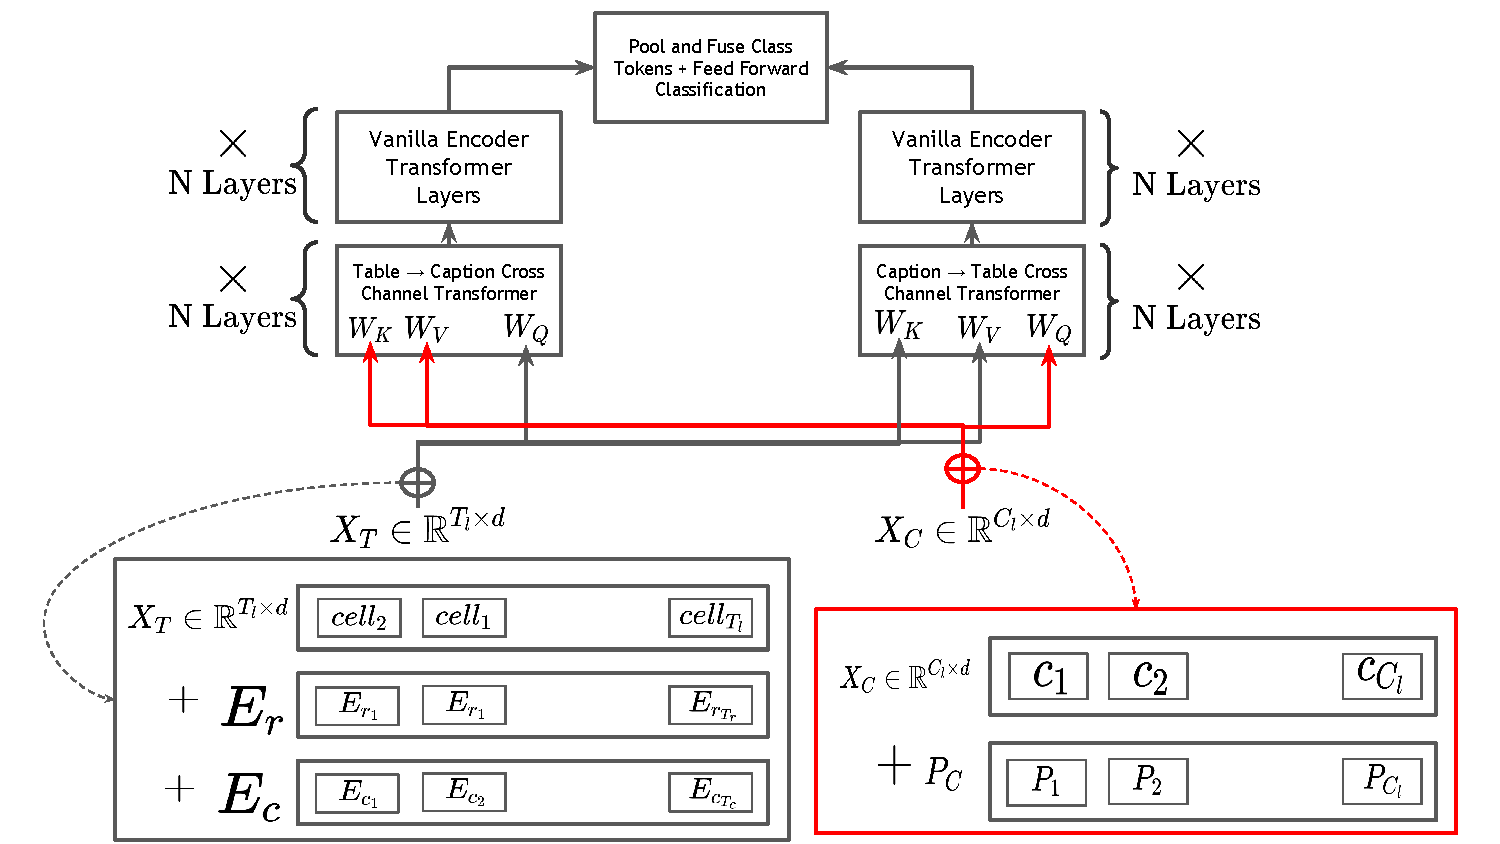
\includegraphics[width=\maxwidth{\textwidth}]{src/images/Pic-Export-CC-Trans-Thesis.pdf}
    \caption{Cross Channel Transformer For Table Classification. }
    \label{figure\arabic{figurecounter}}
\end{figure}
\refstepcounter{figurecounter}

Based on the models developed by \cite{tsai2019multimodal} and \cite{deng2020turl}, a structurally-aware cross channel Transformer model is adapted to fit the function $f_\theta$. Figure \ref{figure19} shows the outline of the model for classification. This model is chosen to validate wheather cross attention based intermediate representations have an influence on the performance of the model or not. 
\subsubsection{Input Representation}
The input representations for $T$ and $C$ are the same as given in Section \ref{table_classification:models:encoder-model:input-rep}


\subsubsection{Model Description}
The table cell sequence $T_{cell}$ and the Caption $C$ are first converted to embeddings $X_T, X_C$ respectively. Post creation of the embeddings,  the caption embedding  $X_C$ is summed with the position embedding $P_C$; The cell embeddings $X_T$ are summed with $E_r,E_c$. After the summings of the respective embeddings, differentiable CLS tokens are concatenated to $X_T,X_C$.
These embeddings are passed to separate cross channel attention transformer layers \parencite{tsai2019multimodal} after which they are passed to the vanilla transformer encoder attention layers \parencite{vaswani2017attention}. Different strategies are chosen for handling the output of the vanilla tranformer encoder based on the type of task. 

Embeddings at the CLS token position, are pooled from the sequences and concatenated for the table of comparison classification task. Once concatenated, this joint embedding is passed to feed forward layers for classification using Cross Entropy Loss. For the pretaining task, the last vanilla encoder layer’s output will be used for predicting the masked tokens of the input table cells $T_{cell}$ and the caption $C$.

\subsection{Finetuning Scibert Transformer Model}
\cite{beltagy2019scibert} created a model which was trained on large full text corpus of scientific research containing 1.14M research papers. As this model has been subjected large amounts of pretraining, it is chosen for fine-tuning for the same problem as the model may have encountered data of a similar distribution. 
\subsubsection{Input Representation}
\label{table_classification:models:sb:input_rep}
For the finetuning of SciBert, The Table $T$ and caption $C$ are serialized to strings and one concatenated string is created. An example representation is given below: 
\begin{verbatim}
    CAPTION : Table 1: Feature extraction time (Seconds), 
    number of parameters (Millions), and network size (Megabytes) 
    for each source on Office + Caltech-10 datasets.

    TABLE :                          0         1           2      3
0                     Task  Net size  Parameters   Time
1          Squeezenet [17]        46        1.24   13.3
2             Alexnet [21]       227          61   13.9
3           Googlenet [40]        27           7   15.9
4          Shufflenet [51]       6.3         1.4   17.0
5            Resnet18 [15]        44        11.7   14.8
6               Vgg16 [36]       515         138   33.6
7               Vgg19 [36]       535         144   37.1
8         Mobilenetv2 [35]        13         3.5   21.4
9        Nasnetmobile [55]        20         5.3   39.3
10           Resnet50 [15]        96        25.6   22.7
\end{verbatim}

\subsubsection{Model Description}
The input representation string is converted to a sequence of integer tokens which are capped to the length of 512 tokens because of SciBert's constraint on maximum sequence length. A class token is appended at the start of the sequence; the sequence is then passed to the Scibert Model. The class token is pooled from after the final layer and is passed to a feed forward neural network for binary classification using cross entropy loss. 


\subsubsection{Model Training}
The model is trained using the for 6 epochs with a linear learning rate warm up schedule of 20 epochs.

\subsection{Caption only Encoder Transformer}

\subsubsection{Input Representation}
The input representation for the Caption only Encoder Transformer uses only the Caption $C$ as input. The encoder and the input representations for the transformer is same given in Section \ref{table_classification:models:encoder-model:input-rep} and Figure \ref{figure18}.

\subsection{SVM and Naive Bayes}
SVM models are used as baselines as when \cite{kim2012scientific} conducted a study for table type classification, deep learning was not as popular. Naive Bayes(NB) model are also chosen as an additional baseline for the classification task. 

The input representation for the SVM and the NB model are the same as the string described in Section \ref{table_classification:models:sb:input_rep}. The string undergoes tokenisation and a classifier is trained based on TF/IDF values of the input strings. 

\subsection{Pretraining Transformers}
\label{table_classification:pre-train}
Based on the insights learned from \cite{hernandez2021scaling} on the effectiveness of pretrained models for downstream tasks, both transformer models in Section \ref{table_classification:models:cross-channel} and Section \ref{table_classification:models:encoder-model} are first pretrained with 70K tables from papers from ArXiv. The pretraining consists of the task of Mask Language Modeling(MLM) for the sequence of cells $T_{cell}$ and the caption $C$. The model is tasked to predict the token where a MASK token is inserted in the table $T$ and caption $C$. A mask is inserted in 80\% of the training samples with 15\% of the sequence being masked. The cross entropy losses from MLM losses of the Table and Caption are summed and backpropagated. The pretraining task for the CCT and E-MCT transformer models is run for 35K steps in 5 epochs.

The caption only transformer is trained with MLM loss on the captions for 6K steps over 5 epochs. It is trained for lesser steps due to larger batch size. The loss of the pretaining for the caption only transformer can be seen from Figure \ref{figure22}. 

The learning rate for all pretraining tasks is set to 0.0001 with an AdamW \parencite{loshchilov2017decoupled} optimizer. 

\subsection{Training Transformers For Classification}
\label{table_classification:models:class-task}
After CCT ,E-MCT and the caption only Transformer undergo the pretraining task, the transformer layers from the models are extracted; A new linear classifier head is added as the last layer and then the models are finetuned on the classification task with a learning rate (LR) of 2e-05, scheduled with a linear LR scheduler for 20 epochs using the AdamW optimizer. All models trained for classification undergo same conditions for training. Even the model trained from scratch on the classification task undergo the same optimization regime for same number of epochs.  

\section{Dataset Collection, Labeling and Construction}
\label{table_classification:data-coll}

\begin{figure}[h]
    \centering
    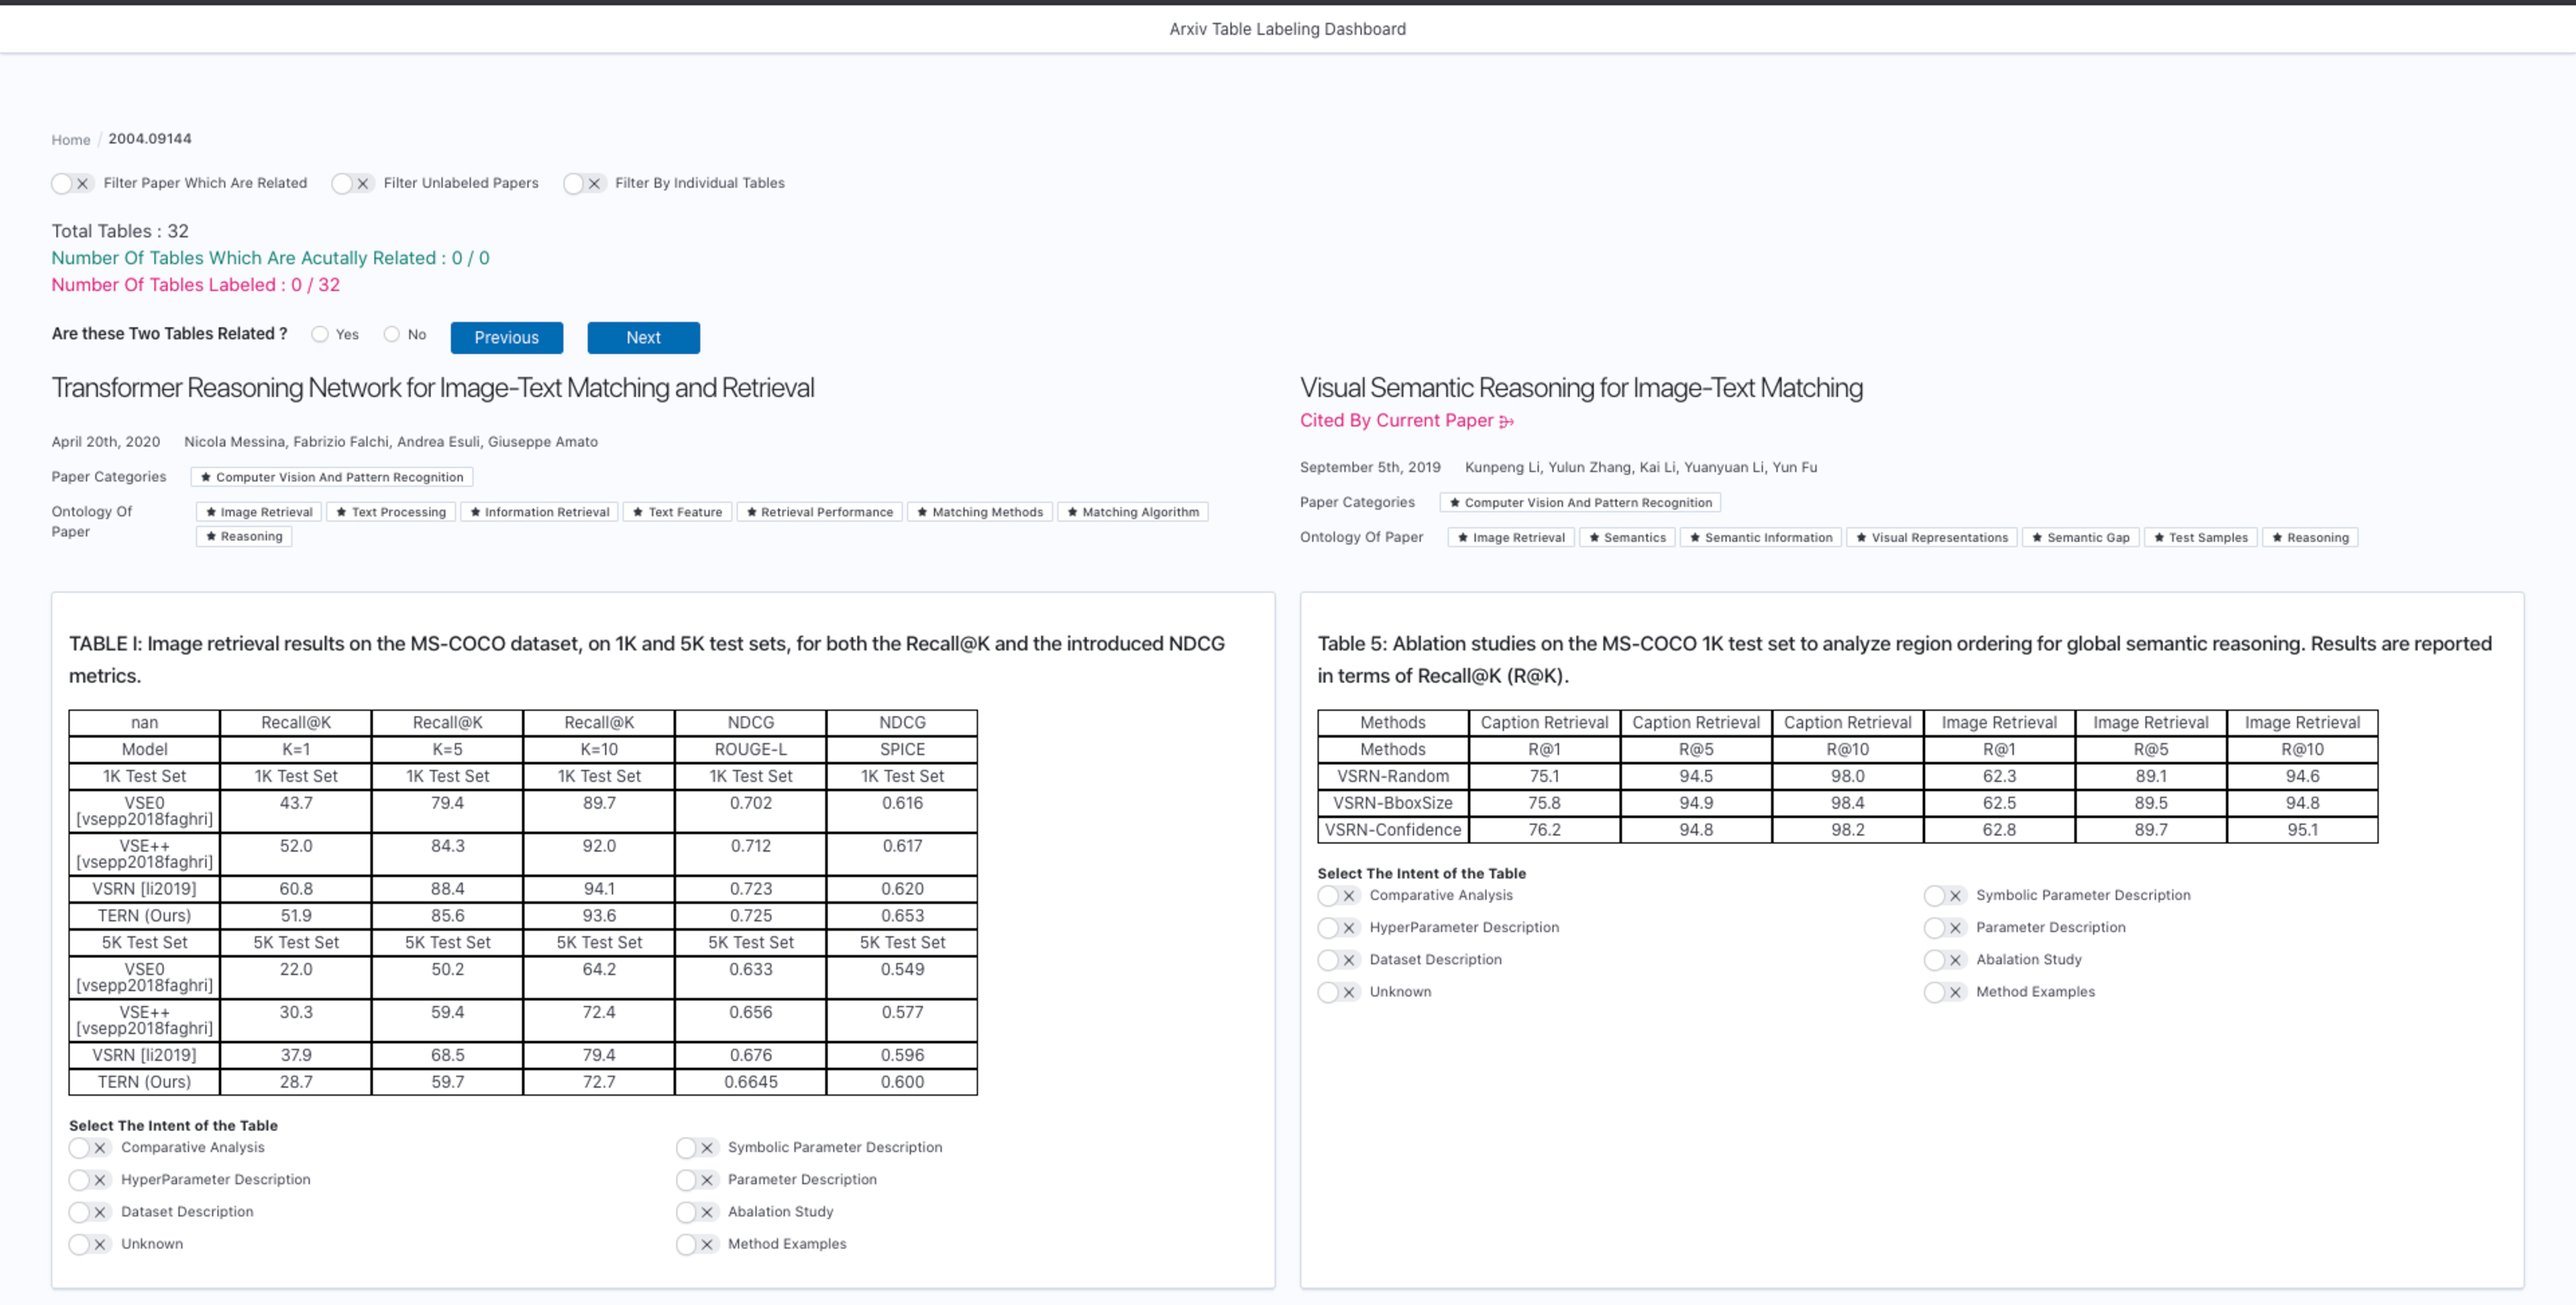
\includegraphics[width=\maxwidth{\textwidth}]{src/images/table-lable-exp.pdf}
    \caption{Table Labeling Interface For Table Relation and Type Annotation. }
    \label{figure\arabic{figurecounter}}
\end{figure}
\refstepcounter{figurecounter}

\subsection{Data Collection}
\label{table_classification:data-coll:coll}
All the tables needed for classification are extracted from the LaTeX source via Sci-Genie. Sci-Genie uses arxiv-vanity/engrafo\footnote{https://github.com/arxiv-vanity/engrafo} to convert LaTeX to HTML. The tables are extracted from HTML using CSS selectors. The LaTeX to HTML conversion ensures specific CSS selectors for explicitly stated tabular data in the LaTeX source. Once the tables are extracted from the HTML source, they are serialized to pandas DataFrames and stored in the search index. The schema of the stored data is described in Chapter \ref{sci-genie-core:data-layer:table-index}. 

\subsection{Data Labeling}
\label{table_classification:data-coll:lab}
\begin{figure}[h]
    \centering
    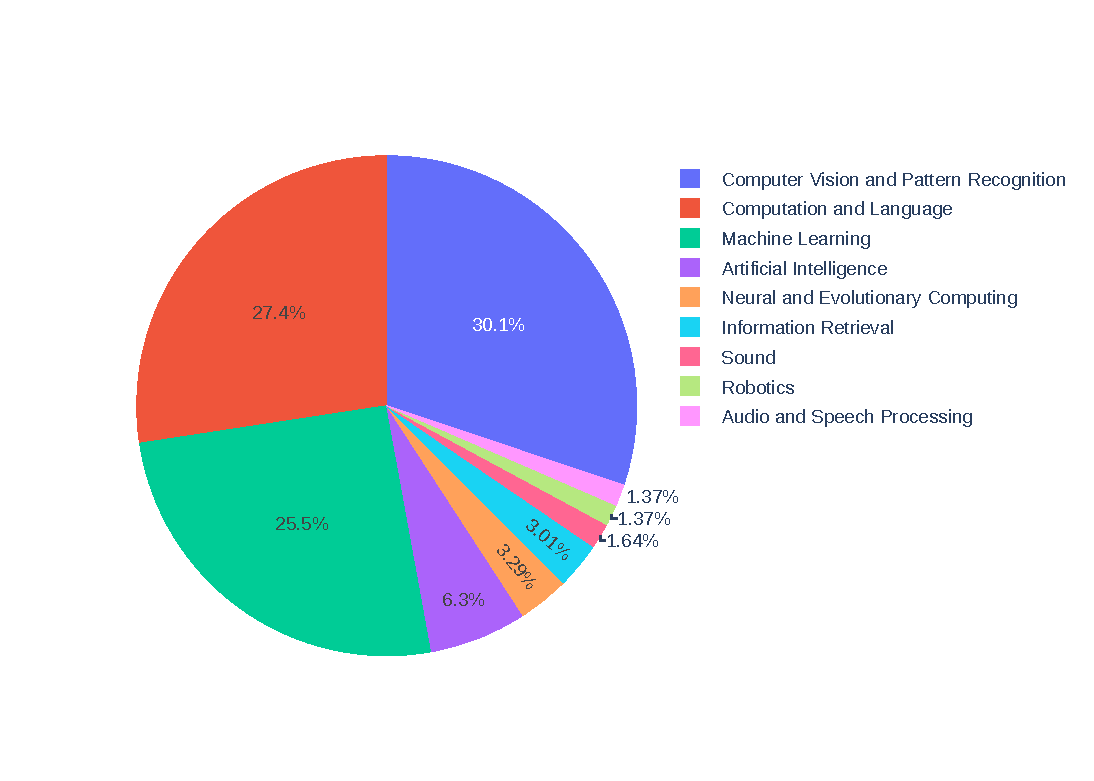
\includegraphics[width=\maxwidth{\textwidth}]{src/images/labeled_data_distribution.pdf}
    \caption{Distribution of the different categories of papers the labeled tables belongs to.}
    \label{figure\arabic{figurecounter}}
\end{figure}
\refstepcounter{figurecounter}

\begin{figure}[h]
    \centering
    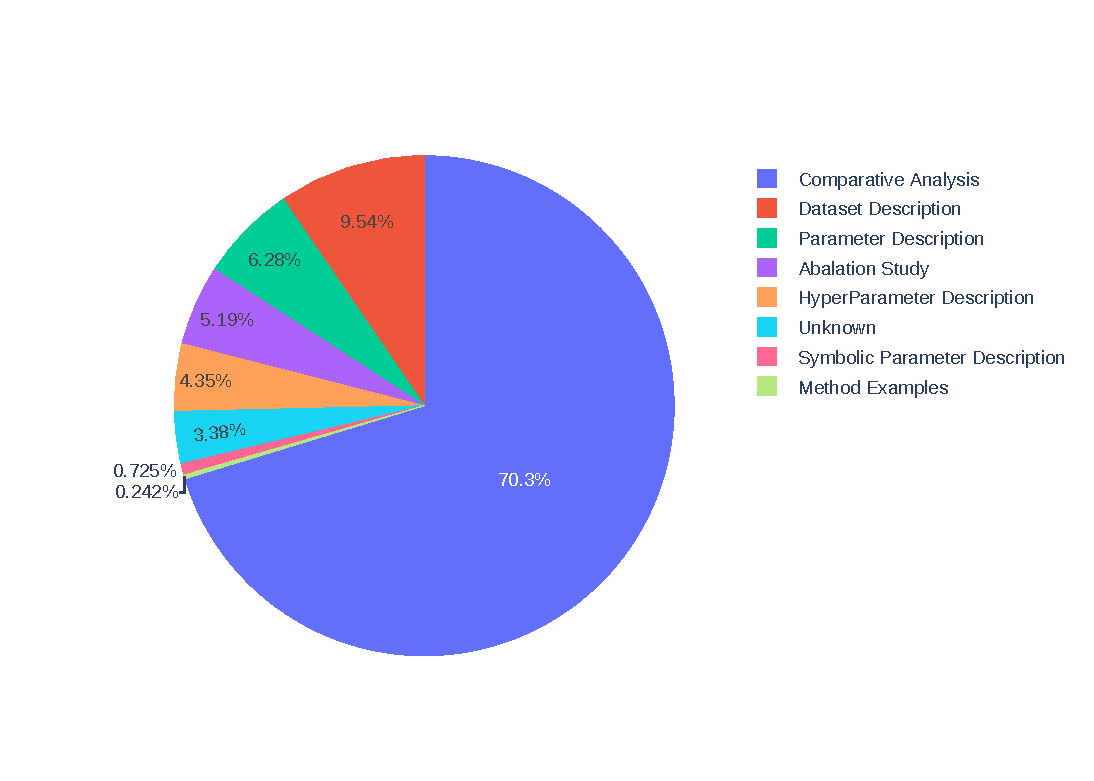
\includegraphics[width=\maxwidth{\textwidth}]{src/images/labeled_intent_distribution.pdf}
    \caption{Distribution of the labeled types for different tables identified in the labeling process.}
    \label{figure\arabic{figurecounter}}
\end{figure}
\refstepcounter{figurecounter}
A labeling interface (Figure \ref{figure20}) is designed to annotate table types. Tables are annotated from 240 research papers. The papers are chosen at random to label. The topics of the papers from which the tables are derived can be seen in Figure \ref{figure21}. To explicitly discover tables which are \textit{not} describing comparisons, the following types of tables are defined: 
\begin{itemize}
    \item Comparative Analysis : The table is describing a comparison between entities based on some metric/metrics. This is the type of table the classifier is supposed to classify.
    \item Symbolic Parameter Description : The table is describing some symbols which could belong to an equation.
    \item HyperParameter Description : The table is describing hyper parameters for some experiment.
    \item Dataset Description : The table is describing statistics/examples from some dataset. 
    \item Ablation Study : The table is describing ablation study or showing some perturbation analysis.
    \item Parameter Description: The table is describing parameters or entities which are relevant to describing the experiment. The label is more generalised than HyperParameter Description or Dataset Description or Symbolic Parameter Description. This label is provided when labelers are unable to categorize a table under a HyperParameter Description or Dataset Description or Symbolic Parameter Description but do observe a form of parametric description necessary to describe an experiment.  
    \item Method Examples : These are tables which are showing input-ouput of some method described in the paper. These types of tables are observed in Machine learning papers where authors show samples various input-output pairs of for an ML model.
\end{itemize}
The above defined types are similar to \cite{kim2012scientific} but also help capture some types which are observed distinctly in recent CS literature. The tables which could not be explicitly classified are labeled as \textit{Unknown}. Examples of all tables are provided in the Appendix \ref{appendix:toc:type-exp}. The extra types are added during the labeling phase to ensure a solid justification for a label when a labeler chooses to label a table. 

3 labelers are tasked to label the data. 820 tables are labeled out of which 574 tables are describing a comparison and 246 are not. Figure \ref{figure22} visualizes the distribution of the labeled types of tables as a pie chart. 

\subsection{Test Set Construction}
\label{table_classification:data-coll:test}
The test set consists of 100 tables describing comparisons and 100 tables which are not describing a comparison. 100 random samples are extracted from tables which are labeled "Comparative Analysis". 100 random samples are taken from tables belonging to the other classes. 

\subsection{Training Set Construction}
The training set consists of the 620 tables which remain after the extraction of the test set. As the dataset has a class imbalance, the classes are rebalanced by duplicating data of non-comparison-tables for the classification training process. 
\pagebreak
\section{Experiment Results}
\label{table_classification:experiment-result}

\begin{table}[h]
    \label{table\arabic{tablecounter}}
    \centering
    \begin{tabular}{llllr}
        \toprule
                         Model Name &                 Loss &             F1 Score &               Accuracy \\
        \midrule
          Caption Only without Pretraining &  $ 0.599 \pm 0.017 $ &    $ 0.7134 \pm 0.001 $ &     $ 71.354 \pm 0.01 $ \\
          Caption Only with Pretraining  &  $ 0.676 \pm 0.036 $ &  $ 0.757 \pm 0.086 $ &   $ 73.438 \pm 8.854 $ \\
          E-MCT without Pretraining &  $ 0.567 \pm 0.003 $ &  $ 0.809 \pm 0.016 $ &   $ 80.404 \pm 1.765 $ \\
          \textbf{E-MCT with Pretraining} &  $ \mathbf{0.417 \pm 0.044} $ &  $ \mathbf{0.845 \pm 0.017}$ &  $\mathbf{84.505 \pm 1.722}$ \\
          CCT without Pretraining &   $ 0.658 \pm 0.13 $ &  $ 0.596 \pm 0.144 $ &  $ 63.281 \pm 14.844 $ \\
          CCT with Pretraining &  $ 0.505 \pm 0.008 $ &    $ 0.7962 \pm 0.001 $ &     $ 79.688 \pm 0.01 $ \\
          SciBERT Finetuning &  $ 0.528 \pm 0.013 $ &  $ 0.826 \pm 0.005 $ &   $ 82.292 \pm 0.521 $ \\
          SVM &  -  &  $ 0.77 \pm 0.007 $ &   $ 74.635 \pm 0.991 $ \\
          Naive Bayes &  -  &  $ 0.77 \pm 0.007 $ &   $ 73.125 \pm 1.06 $ \\
        \bottomrule
    \end{tabular}
    \caption{Test set results of the table of comparison classification models. The presented statistics are after averaging 8 training runs. }
\end{table}
\refstepcounter{tablecounter}

The following are the ML models whose results are reported in Table \ref{table5}:
\begin{itemize}
    \item Cross Channel Transformer (CCT) With/Without pretraining. 
    \item Encoder Only Multi-Channel Transformer (E-MCT) With/Without pretraining. 
    \item Caption Only Transformer Encoder With/Without pretraining. 
    \item SciBert Finetuned on the classification task (Baseline). 
    \item SVM and Naive Bayes (Baseline). 
\end{itemize}


\begin{figure}[h]
    \centering
    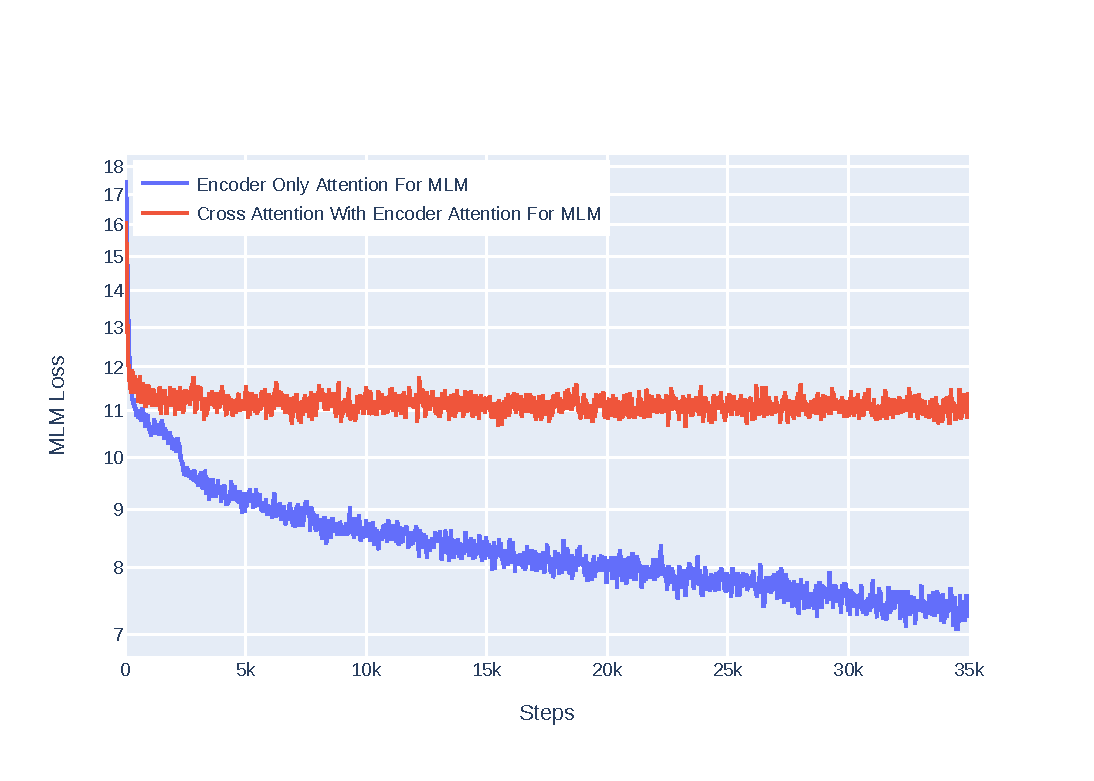
\includegraphics[width=0.8\maxwidth{\textwidth}]{src/images/mlm-loss-comparison.pdf}
    \caption{Masked Language Modeling(MLM) Loss For Encoder Style Attention VS Cross Attention. The MLM losses for $T$ and $C$ are summed. }
    \label{figure\arabic{figurecounter}}
\end{figure}
\refstepcounter{figurecounter}

\begin{figure}[h]
    \centering
    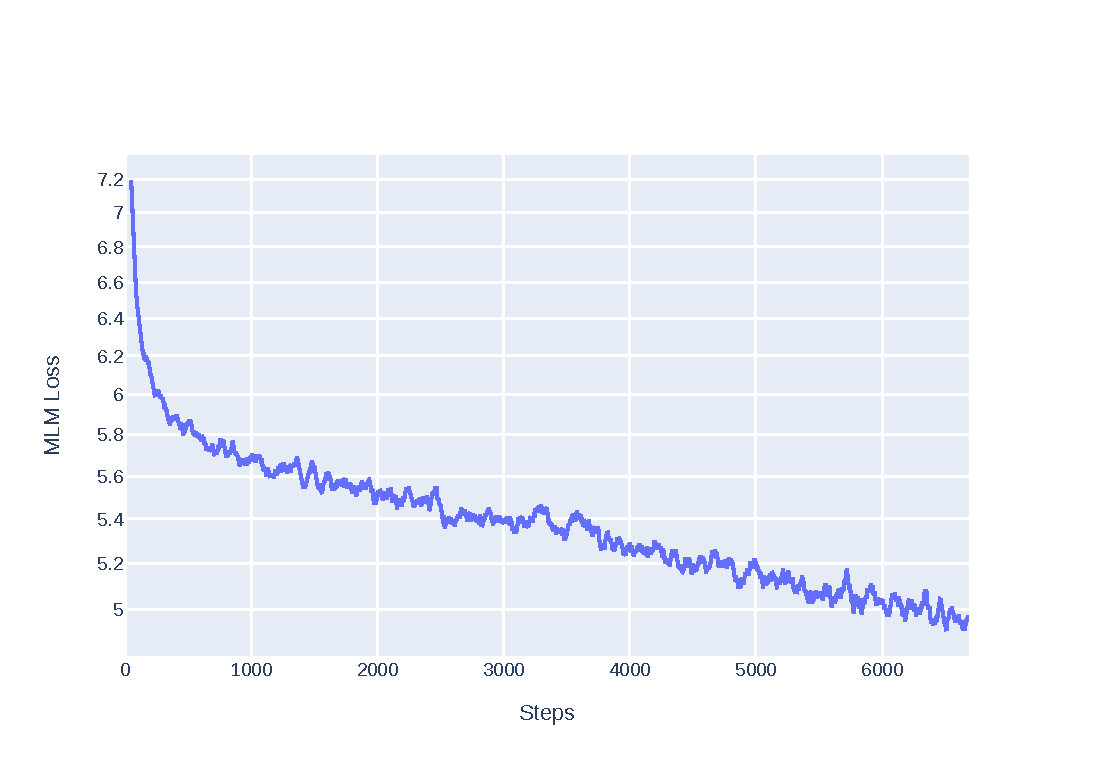
\includegraphics[width=0.8\maxwidth{\textwidth}]{src/images/mlm-loss-comparison-caption.pdf}
    \caption{Masked Language Modeling(MLM) Loss For Caption Only Transformer Encoder Model }
    \label{figure\arabic{figurecounter}}
\end{figure}
\refstepcounter{figurecounter}
\FloatBarrier
All experiments are conducted using Google Colab Notebooks on NVIDIA P100 GPUs. The models that undergo pretraining follow the pretraining regime given in Section \ref{table_classification:pre-train}. The loss plot for the pretraining phases for the E-MCT ,CCT, Caption only transformer are visualized in Figure \ref{figure23}, \ref{figure24}. 

All model variants except for SciBert are trained for 20 epochs. SciBert is trained for 6 epochs. The training optimization details are provided in Section \ref{table_classification:models:class-task}. 

The optimization method is kept the same for all classification experiments.  More details on the hyperparameters for the experiments are found in the Appendix \ref{appendix:toc}.  

All experiments are conducted on the same frozen test set with evenly balanced samples as described in Section \ref{table_classification:data-coll:test}. Table \ref{table5} describes performance on test set for each model after averaging 8 training runs. 

A more detailed view of the test set performance metrics can be seen from Figure \ref{figure27}.  Figure \ref{figure27} visualizes the distribution of performance metrics described in Table \ref{table5}. Figure \ref{figure25}, \ref{figure26} visualize the metrics like loss, accuracy and F1 score during the training process for all the models. 

The metric value at each training step within the plots of Figure \ref{figure25} and \ref{figure26} is an average from the 8 experiment runs. Section \ref{table_classification:experiment-result:result-discussion} discusses the insights inferred from the experiment results. 

\pagebreak
\begin{figure}[p!]
    \centering
    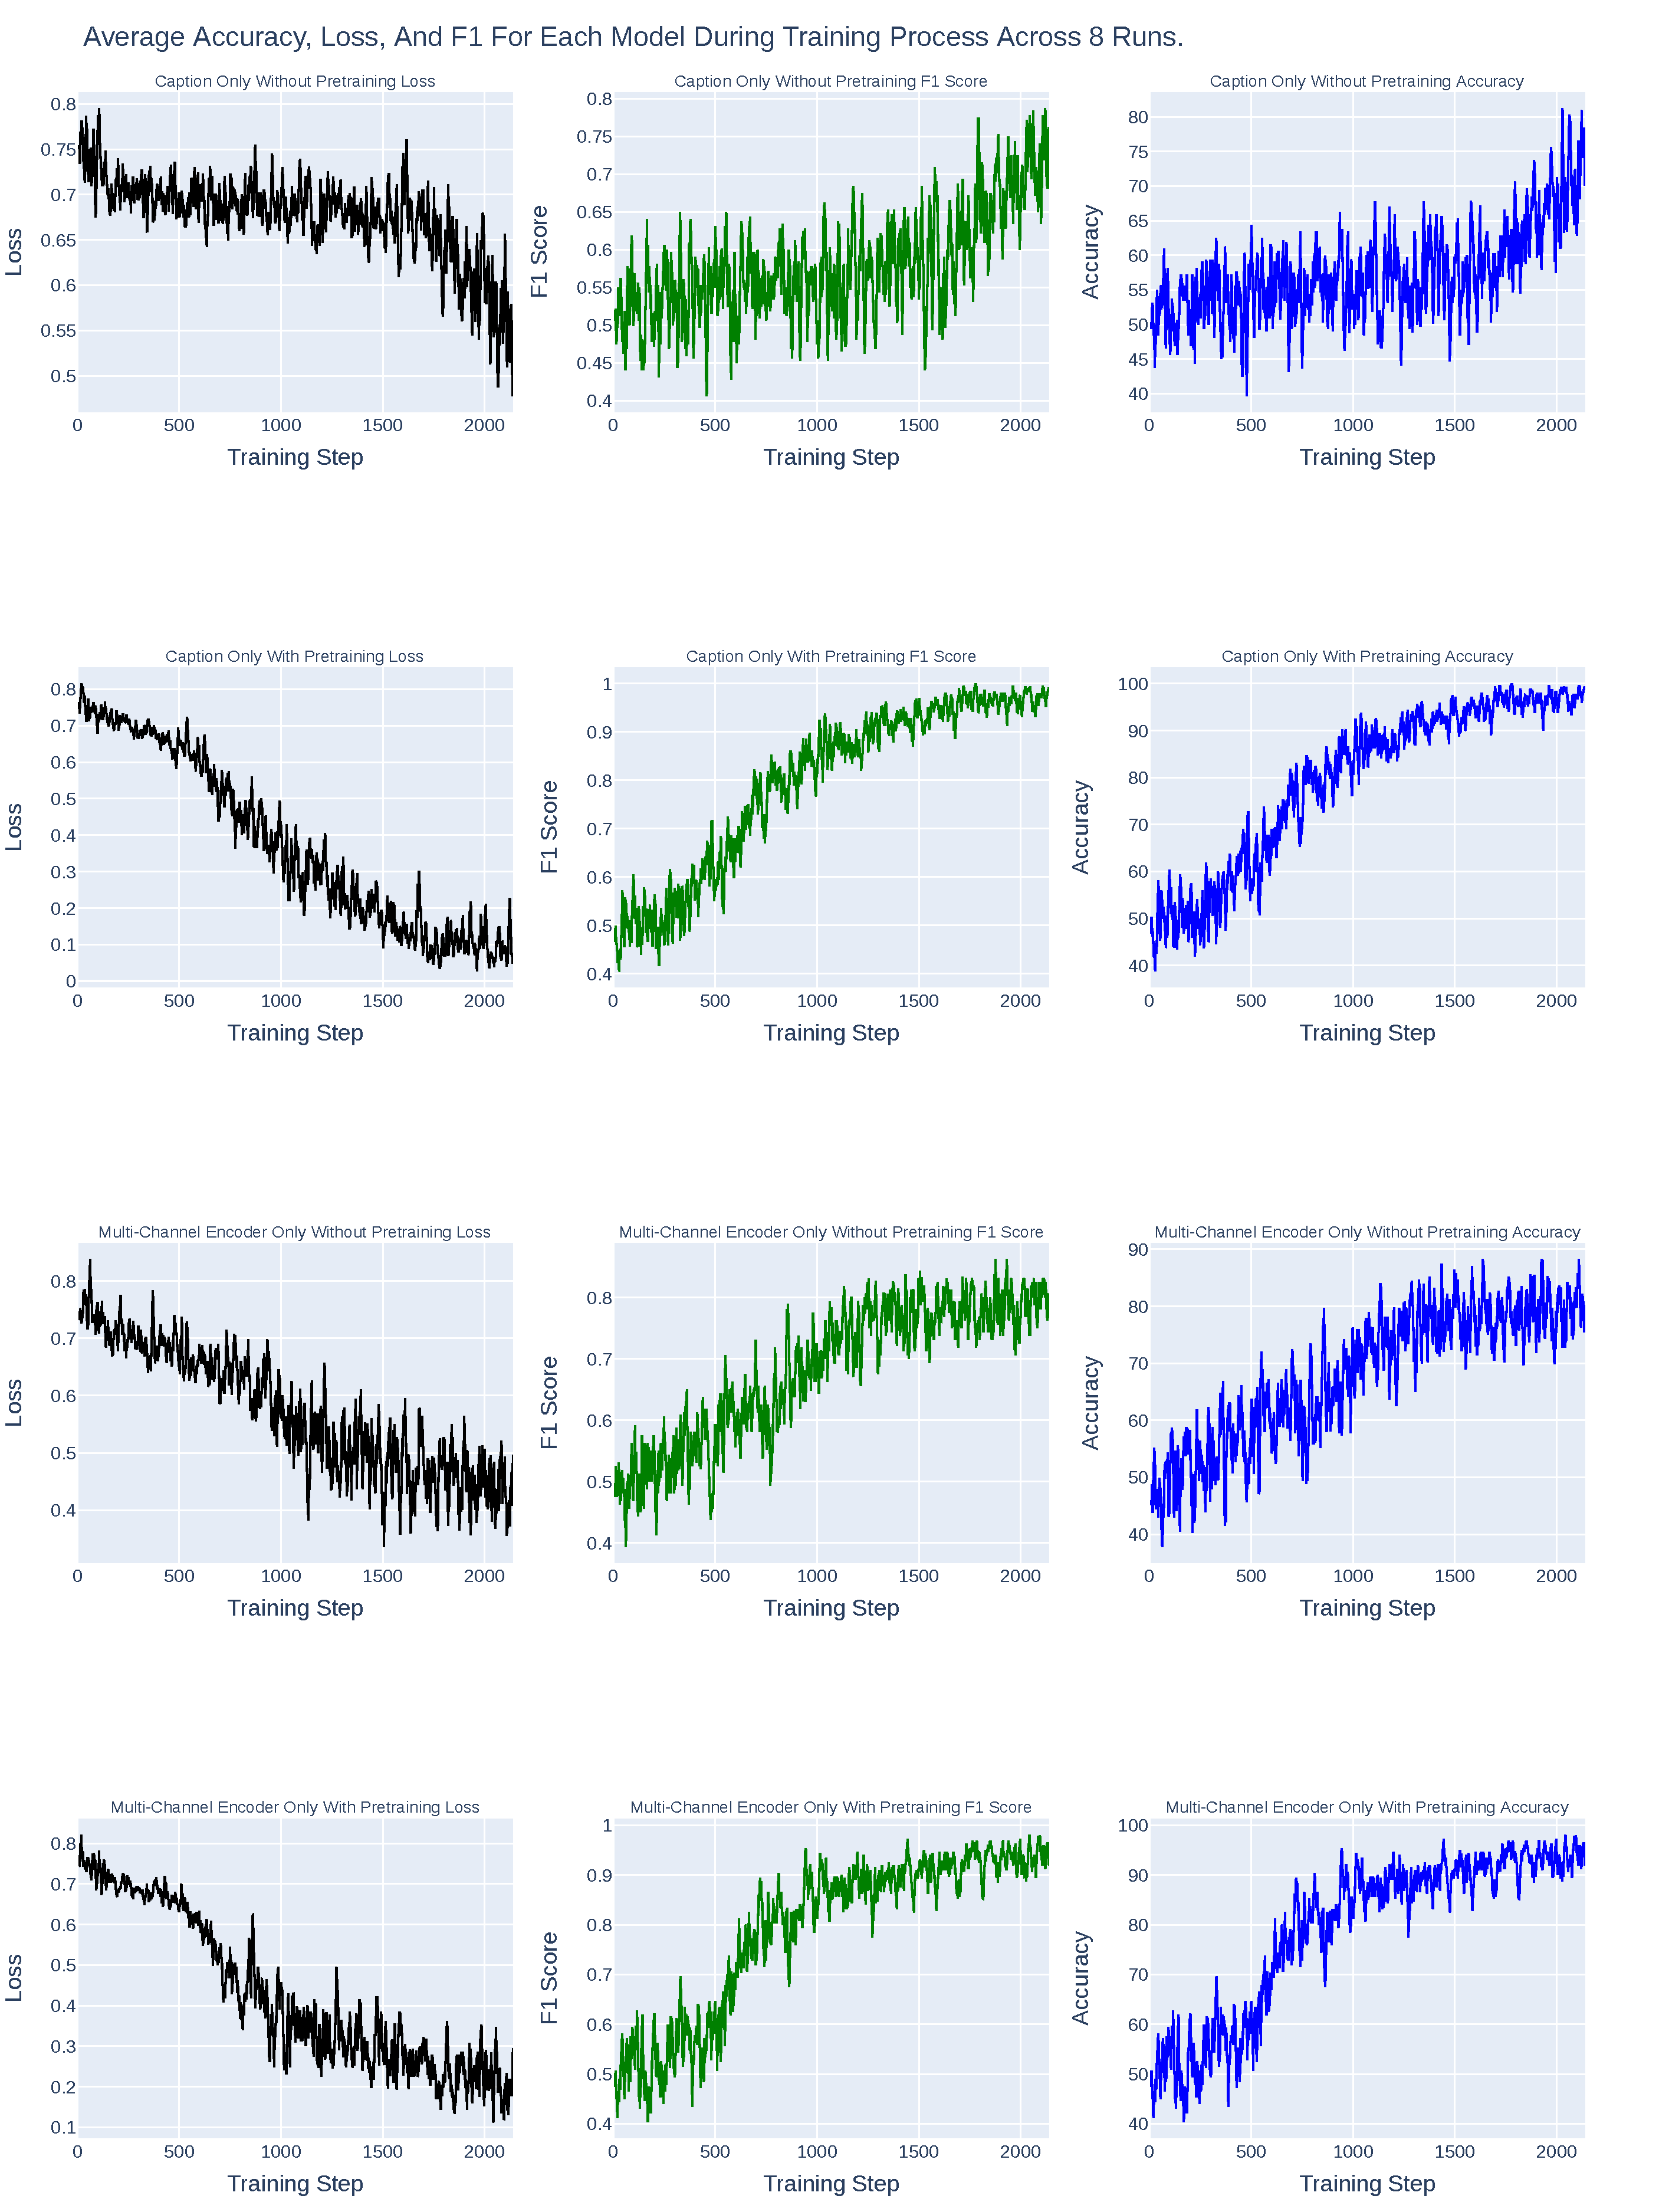
\includegraphics[width=0.96\maxwidth{\textwidth}]{src/images/Loss-Distriubiton-Train-Set-1.pdf}
    \caption{Average training loss, accuracy and F1 scores during the training process for the classification task across 8 runs using caption only Transformer with/without pretraining, and the E-MCT with/without pretraining. The metric value at each training step within the plots is an average from the 8 experiment runs.}
    \label{figure\arabic{figurecounter}}
\end{figure}
\refstepcounter{figurecounter}

\begin{figure}[p!]
    \centering
    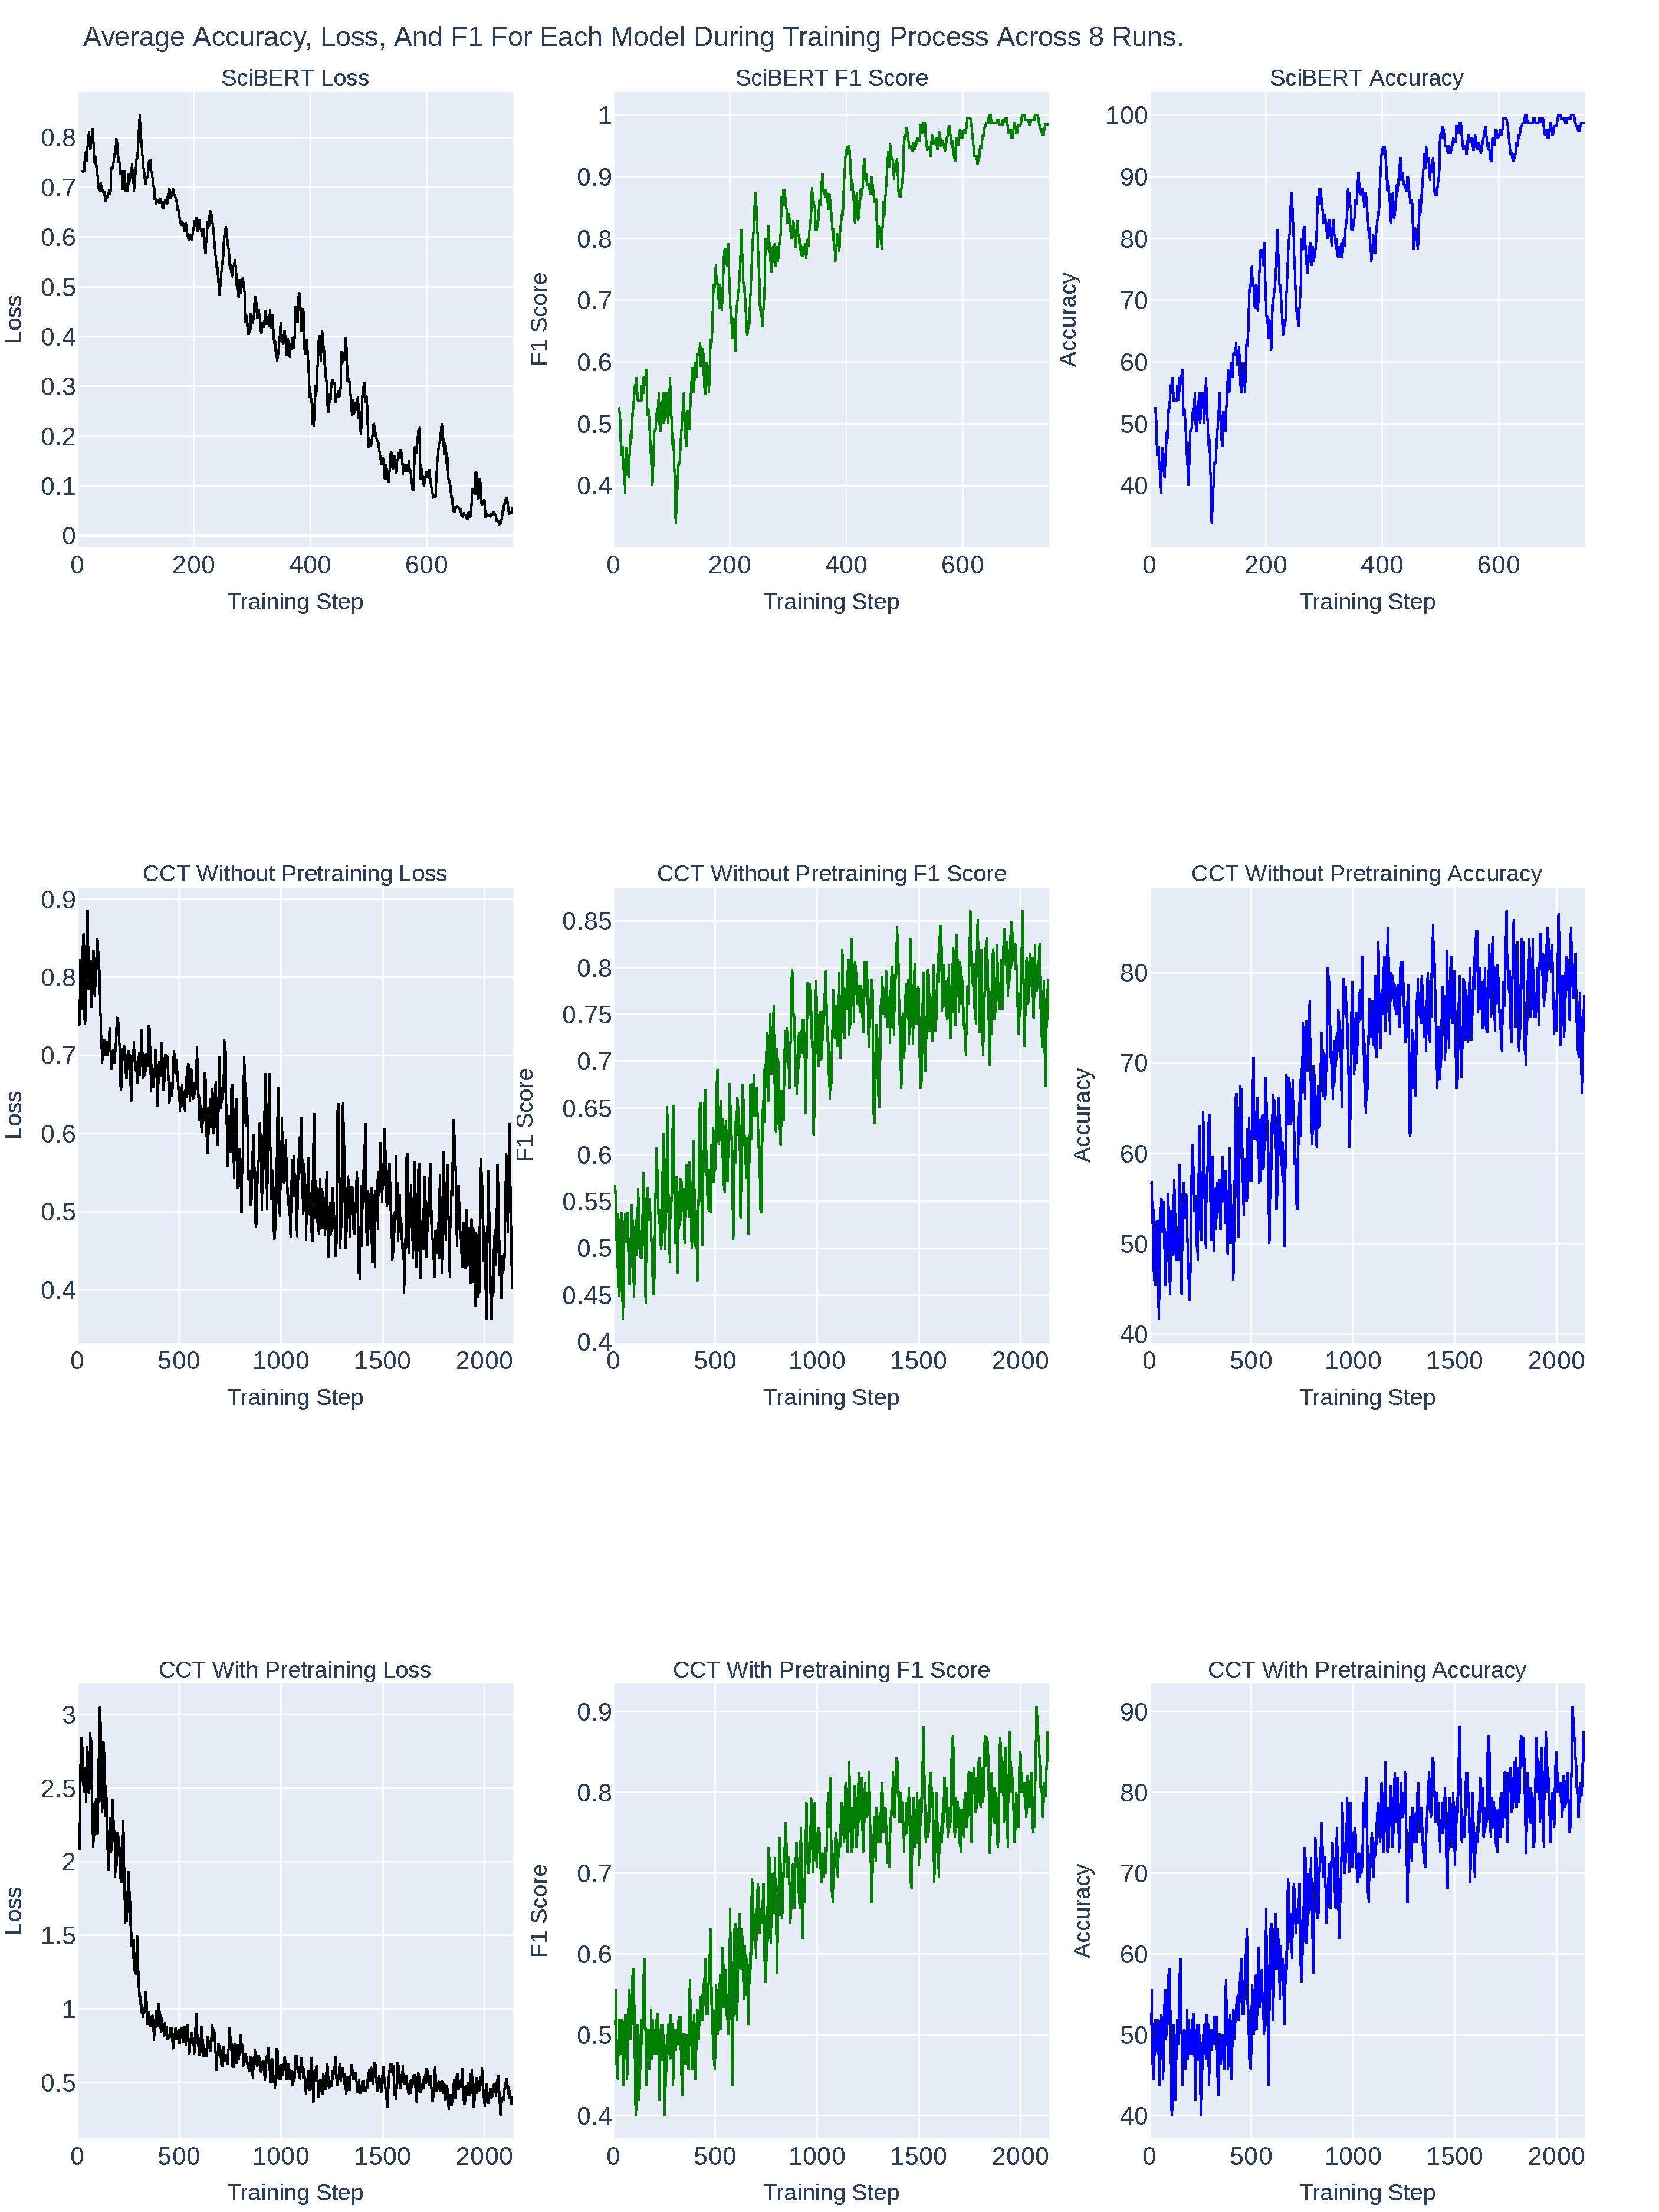
\includegraphics[width=\maxwidth{\textwidth}]{src/images/Loss-Distriubiton-Train-Set-2.pdf}
    \caption{Average training loss, accuracy and F1 Score during the training process for the classification task across 8 runs using CCT with/without pretraining and Finetuning Sci-Bert. The metric value at each training step within the plots is an average from the 8 experiment runs. }
    \label{figure\arabic{figurecounter}}
\end{figure}
\refstepcounter{figurecounter}

\begin{figure}[p!]
    \centering
    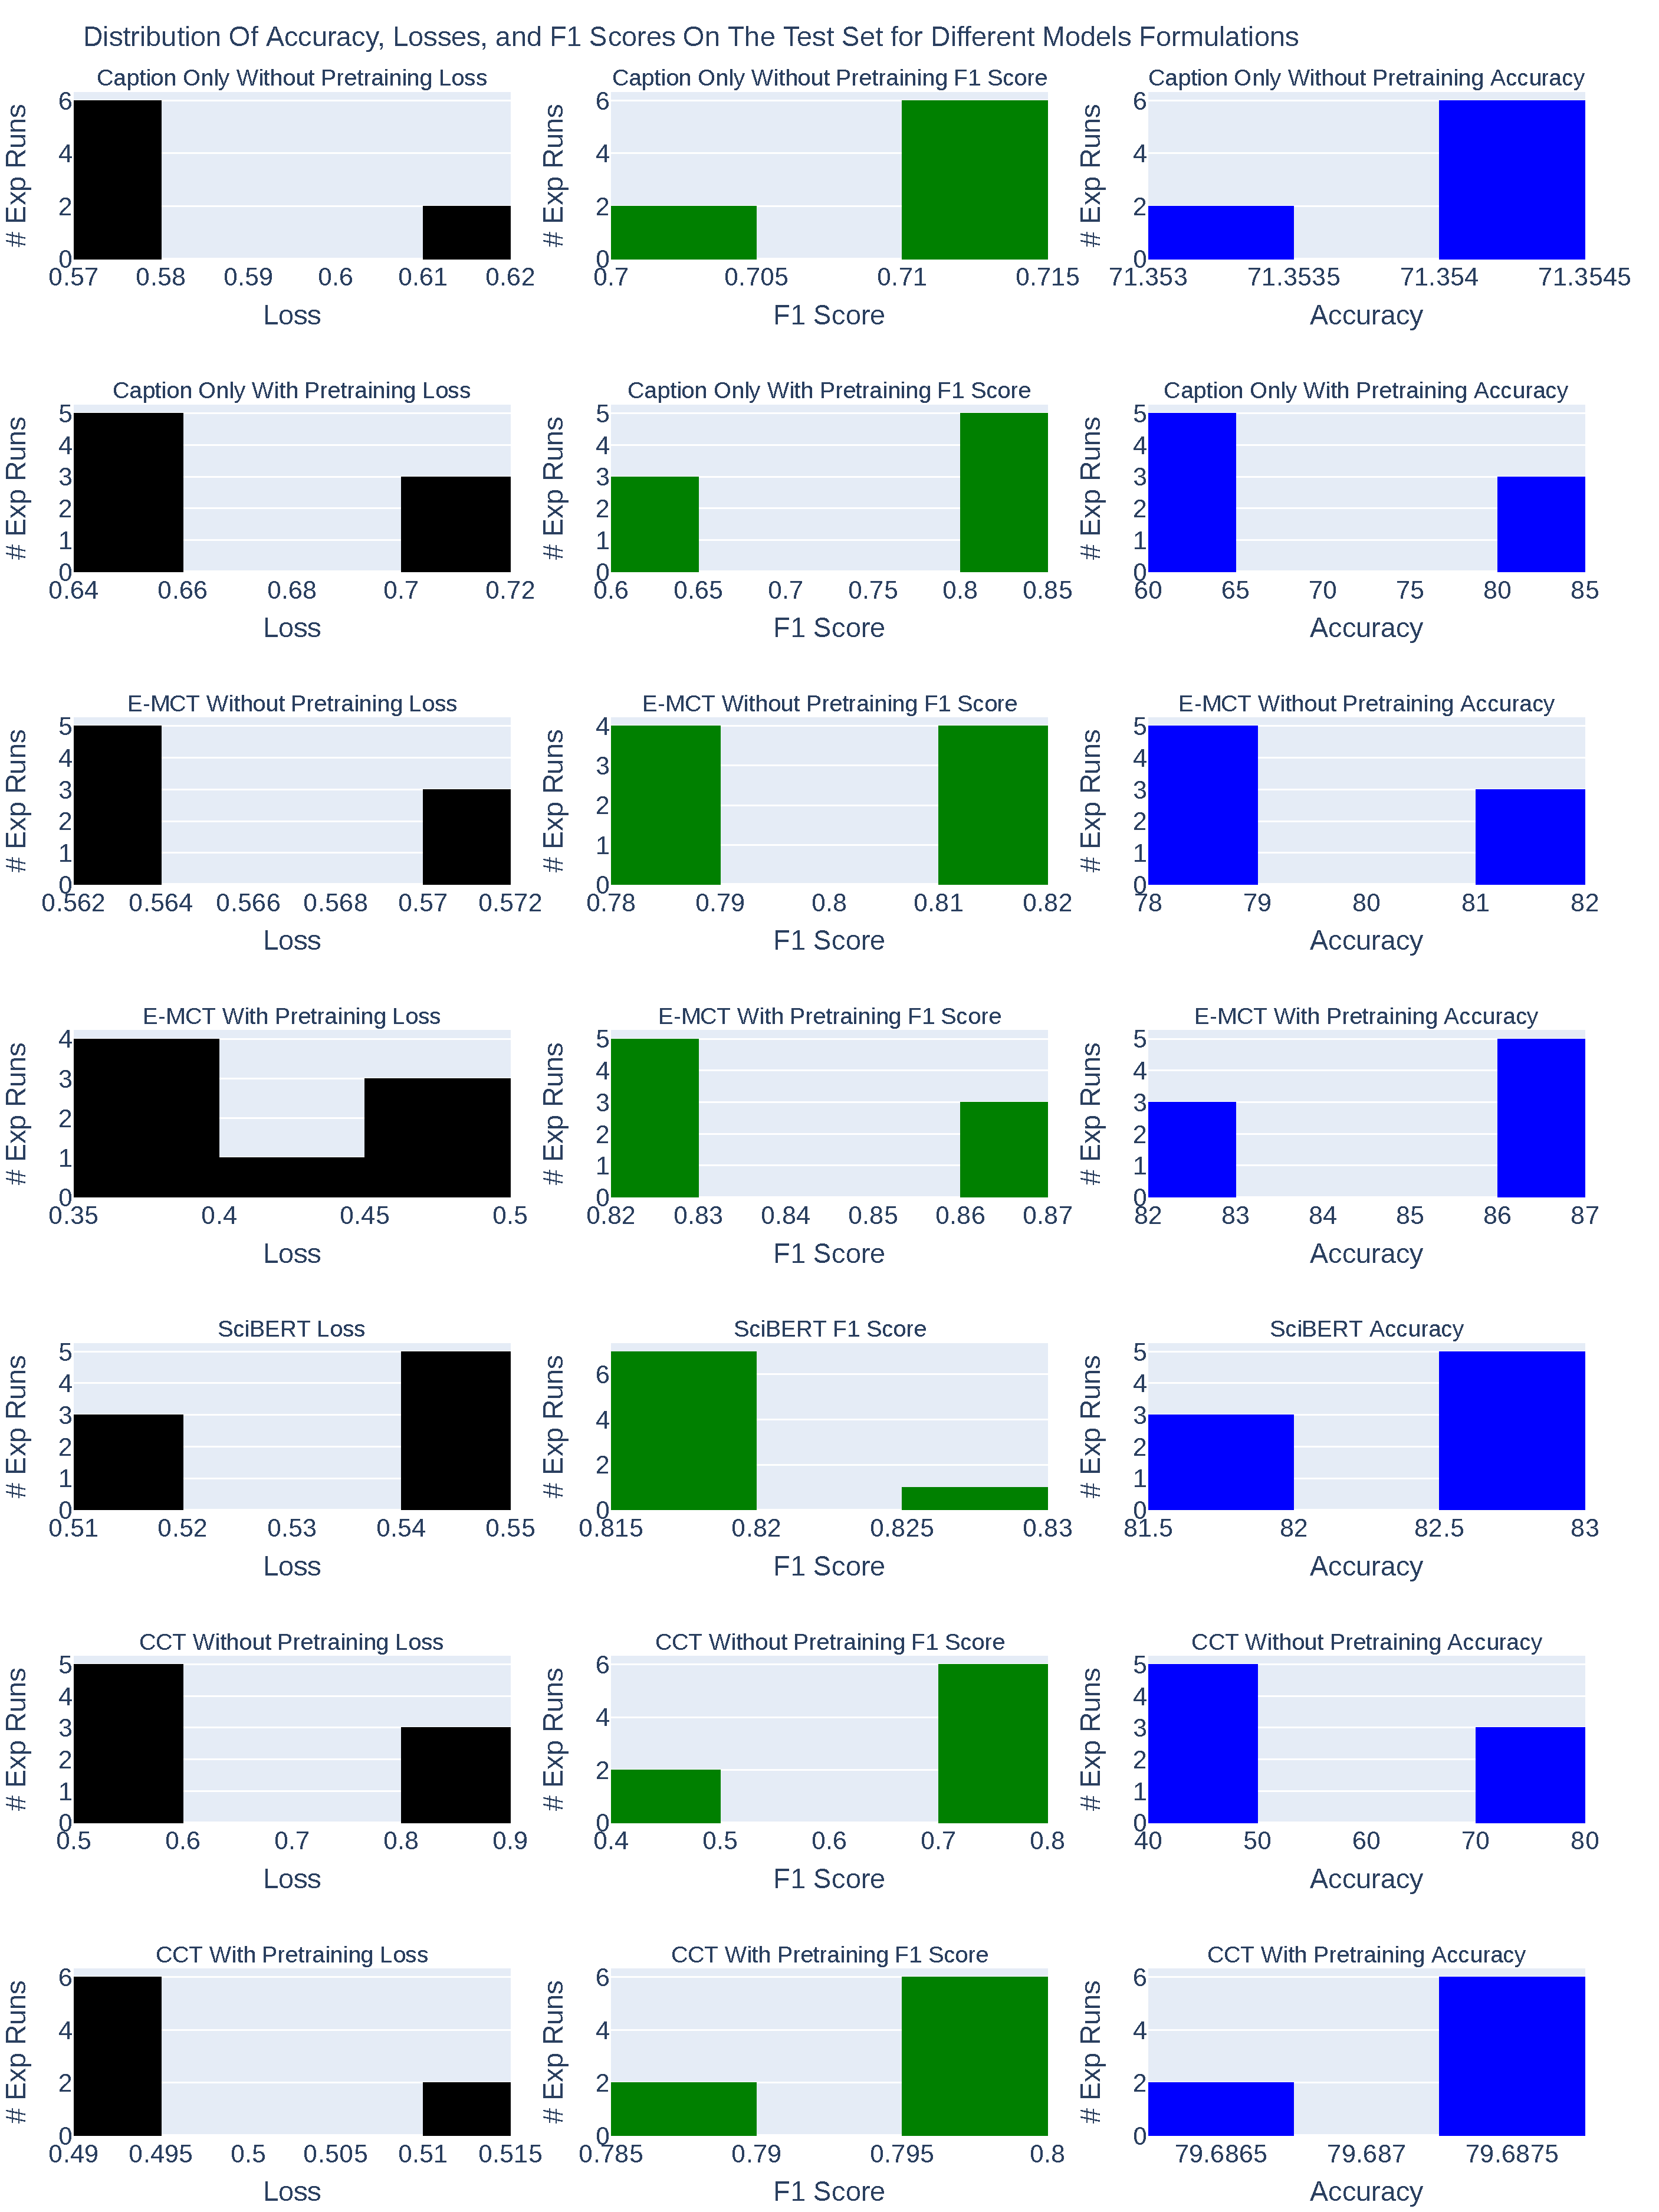
\includegraphics[width=\maxwidth{\textwidth}]{src/images/Metric-Distribution-For-Test-Set.pdf}
    \caption{Distribution of loss, accuracy and F1 score on the test set for the classification task after 8 training runs for all experiments. The X-axis in each plot represents the metric. The Y-Axis is the number of experiment which resulted in the value of the metric}
    \label{figure\arabic{figurecounter}}
\end{figure}
\refstepcounter{figurecounter}

\FloatBarrier

\subsection{Experiment Result Discussion}
\label{table_classification:experiment-result:result-discussion}
There following are some distinct observations after training the models for the classification task:
\begin{itemize}
    \item Pretraining improves the performance of the model on the task specific optimization. 
    \item Using caption only encoder transformer for the classification task gives performance which comes at par with SciBert but with high variance. 
\end{itemize}

\textit{The pertrained E-MCT model has the best performance on the test set} as seen from Figure \ref{figure27} and Table \ref{table5}. Pretraining improves the performance of all the models including E-MCT, CCT and Caption only transformer compared to training those models from scratch as seen from Figure \ref{figure27}. 

The performance of the pertrained CCT transformer is better than the model trained from scratch because the model trained from scratch has high performance variance in the test set as seen in Figure \ref{figure27}. CCT model has a higer loss on the pretraining task than the E-MCT model as seen in Figure \ref{figure23}. This helps infer the reason for the E-MCT's better performance on the fine-tuning task compared to CCT. 

Even though SciBert (Figure \ref{figure26}) has a better accuracy on the train set than E-MCT (Figure \ref{figure25}), E-MCT generalizes better on the test-set.

It can be argued that the difference in performance between Sci-Bert and E-MCT models (only a few percentage points) is a negligible difference due to the size of the test set. But this arguement also sheds light that while E-MCT is a smaller model, it gives performance at par or better than a larger model like SciBert after pretraining. 

The pretrained caption only encoder transformer performs as well as the SciBert but with a high variance as seen in Figure \ref{figure27}. Even though this pretrained model reaches convergence in the training process as seen in Figure \ref{figure25}, its test set performance has high variance and the best model doesn't outperform E-MCT. 